%% * Format settings ****************************************************************
%% paper arrangement and main font size
\documentclass[utf8,twoside, 12pt, titlepage, openright]{report}
%% Paper size and margins
\usepackage[a4paper,top=2cm, bottom=3cm, left=3cm, right=2cm]{geometry}
%% Police
\usepackage{fontspec}
\setmainfont{Times New Roman}
%% Title format
\usepackage{titlesec}
\titleformat{\chapter}[block]
  {\normalfont\fontsize{16}{16}\bfseries\filcenter}{}{1em}{}
\titleformat{\section}
  {\normalfont\fontsize{14}{14}\bfseries}{\thesection}{1em}{}
\titleformat{\subsection}
  {\normalfont\fontsize{12}{12}}{\thesubsection}{1em}{}
\titleformat{\paragraph}
  {\normalfont\fontsize{12}{12}}{}{1em}{}
%% Inter-line
\usepackage{setspace}
\onehalfspacing

%% Indent first paragraph
\usepackage{indentfirst}

%% for blank pages at end
\newcommand{\blankpage}{
\newpage
\thispagestyle{empty}
\mbox{}
\newpage
}

%% Add Chinese support
\usepackage{xeCJK}
\usepackage{ifplatform}
%% For macOS users, the fonts need additional configurations.
\ifmacosx
\setCJKmainfont[BoldFont=STHeiti,ItalicFont=STKaiti]{STSong}
\setCJKsansfont[BoldFont=STHeiti]{STXihei}
\setCJKmonofont{STFangsong}
\fi

% For logbook
\usepackage{tabularx}


%% * Format settings ****************************************************************
%% The amssymb package provides various useful mathematical symbols
\usepackage{amssymb}
%% The amsthm package provides extended theorem environments
\usepackage{amsthm}
\usepackage{amsrefs}
\usepackage{mathrsfs}
\usepackage{amsmath}
\usepackage{bm}
\usepackage{subcaption}
%\usepackage{natbib}
\usepackage{graphicx}

%% The lineno packages adds line numbers. Start line numbering with
%% \begin{linenumbers}, end it with \end{linenumbers}. Or switch it on
%% for the whole article with \linenumbers after \end{frontmatter}.
%\usepackage{lineno}
%\bibliographystyle{model1-num-names}
%\bibliography{sample.bib}

\usepackage[hidelinks]{hyperref}

\begin{document}
\title{Application of Hopfield neural network on the energy-saving robot path finding and robot arm control.}
\author{Jérémie YANG Zhenyu 杨振宇 \\ Student number : 19214064}
\maketitle
\cleardoublepage
\setcounter{page}{1}

\tableofcontents
\newpage
\chapter*{Abstract}
\addcontentsline{toc}{chapter}{Abstract}
\label{sec:abstractEng}

Robots are important tools in nuclear power plants since they could receive radiation without doing
damage other than economy.
It could be foreseen that once a material for robot fabricating that is radiation-resist enough,
robot will be very universal in nuclear power plants.
On the other hand, algorithms controlling the robot will be very important too.
The complicated ground conditions in nuclear power plants require the robot to be able to climb stairs,
avoid or step over various kinds of obstacles and make right decisions for saving energy.


\chapter{Introduction}
\label{cha:introduction}
\section{Literature review}
\label{sec:review}

\section{Choice of technique}
\label{sec:choice}

\section{Projects to implement}
\label{sec:projects}

\subsection{Project 1 - 2D path finding problem}
\label{ssec:project1}

Project 1 consists of using Hopfield neuronal space to find an optimum path from an origin to a destination
on considering energy and time consumption.
\chapter{Hopfield neutral space}
\label{cha:hopfield}

\section{Principles}
\label{sec:hopfield_Principles}

\section{Advantages and disadvantages}
\label{sec:hopfield_advanddisadv}


\chapter{Innovative algorithms to use for the two projects}
\label{cha:algorithm}

\section{Energy-saving path finding}
\label{sec:algorithm_project1}

\section{Multi-arm robot}
\label{sec:algorithm_project2}
In this project, comparing to the first one, some additional steps must be taken.
One is to calculate the robot’s “presence” which means the space occupied in the work space by the robot’s arms in each configuration.
It is necessary for calculating the neuronal space.
Obstacles includes, in addition to all points of the obstacles in XY dimension,
all configurations that the robot’s presence has overlapped space with any obstacles.

These calculations consume lots of computational resources.
So various approaches that can reduce this consumption by thousands of times are proposed in the following chapters.

\subsection{Robot presence calculation}
\label{ssec:algorithm_presence}
The robot arms’ special presence is calculated using two methods.
One is to consider the distance between any point to the arm’s joint and to the arm’s central axis.
The other is to use the equation of robots outer lines.

It is tested that the first one is faster and the result of second one is better.
As we use a pre-calculation approach (introduced in section \ref{sec:optimizaiton_Precalculation}) to reduce the calculation time
in this step there is no need to consider the computational resources consumed in this part.
So we choose the second method.

Based on the joint coordinates, joint angles and arm size, the equations of the robot's arm's outer lines can be obtained.

\subsection{Preparation of neuronal space}
\label{ssec:algorithm_project2_space}
This preparation consists of calculating all the feasible configurations of the robot using the presences calculated.
All neurons of configuration that has overlap with any obstacles are fixed to 0.

This takes fairly amount of time.
So many computational approaches that accelerates the calculation are applied.
The most powerful ones are the usage of Numba and the vectorization. (see chapter \ref{cha:optimizaiton})

\chapter{Optimizations of computer code}
\label{cha:optimizaiton}


\section{Vectorization}
\label{sec:optimizaiton_vectorization}

\section{Numba and code modifications}
\label{sec:optimizaiton_numba}
\subsection{Numba Library}
\label{ssec:numba_numba}
Numba is a Python compiler that transforms Python code to high performance machine code which supports NumPy arrays and functions and loops.
It could also work with CUDA to use Nvidia GPU.

\subsection{Implementation of $np.roll()$ in Numba}
\label{ssec:numba_nproll}
np.roll() was in fact implemented in Numba without support for axis argument.
However, this support is essential for our program. As the code is open source and the merge
commit of this feature can be viewed directly in GitHub, one simple work through is study
and copy those code and add the support for axis.

Let $A$ a matrix of dimension $n$, $B$ the matrix after shifting $shift$ along axis $axis$. 
Then we'll have for all $A[(x_i)_{i<n}], B[((x_i+(i==shift)*shift)\%shape[axis])_{i<n}]=A[(x_i)_{i<n}]$.

In order to prevent $if$ or $for$ overlap which consumes considerable amount of resources, a method using modulus operator is proposed.

Let $a=\prod^{n-axis}_{j=1}shape[n-j],b=\prod^{n-axis-1}_{j=1}shape[n-j]$. Apparently $b=a/shape[axis]$.

The code is not aware of the dimension of the matrix, so we'll have to operate through flatten array (of dimension 1).
A coordinate conversion formula is shown below.

If $A[(x_i)_{i<n}]=A.flat[idx], then idx=\sum^{n-1}_{i=0}x_i\prod^{n-i-1}_{j=1}shape[n-j]$.
So with $B[((x_i+(i==shift)*shift)\%shape[axis])_{i<n}]=A[(x_i)_{i<n}]$, we'll have : 
$$ idx_B=idx_A+((x_{axis}+shift)\%shape[axis]-x_{axis})\prod^{n-axis-1}_{j=1}shape[n-j]$$

Now we've only to get $x_{axis}$ from $idx_A$, firstly by $\%a$, we'll get $\sum^{axis}_{i=0}x_i\prod^{n-i-1}_{j=1}shape[n-j]$.

Then divide by $b$, take only the integer part we'll finally get $x_{axis}$.
The code of this process is shown in figure \ref{fig:nproll}.

\begin{figure}[!htb]
    \centering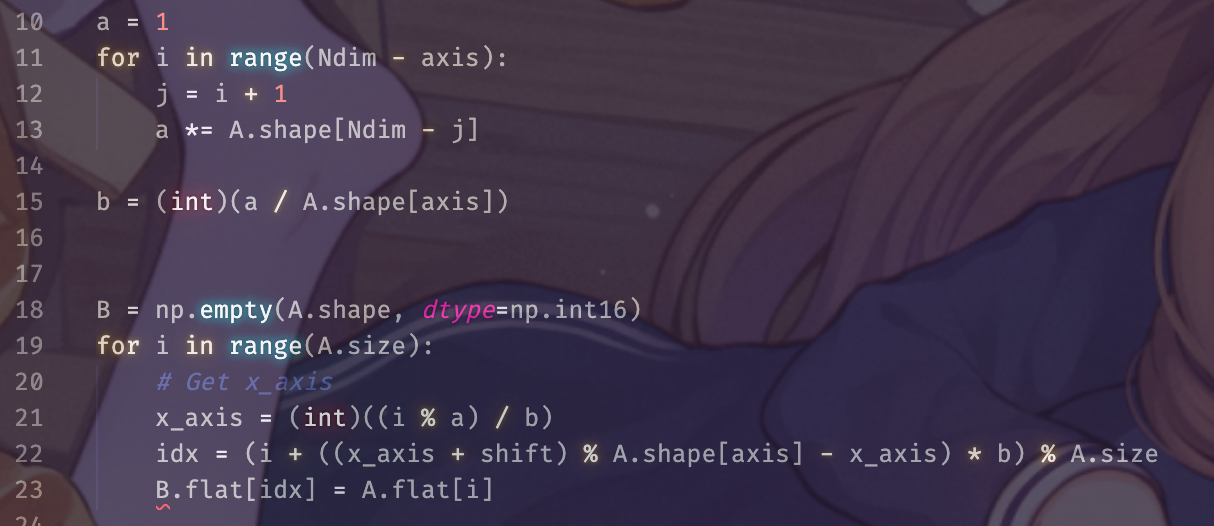
\includegraphics[width=0.6\linewidth]{Figs/implementationOfNpRoll.png}
    \caption{Code of $np.roll()$}
    \label{fig:nproll}
\end{figure}

However, the result of this optimization is not very satisfying. 
In some occasions, the implementation makes the program run slower than without Numba. 

\section{Pre-calculation of robot's coordinates (Project 2 only)}
\label{sec:optimizaiton_Precalculation}

Calculation of the robot's presence (spatial coordinates that the robot occupies) is rather resources expensive.
Since the robot's move in space could be regraded as translation, it could be pre-calculated.
Presences of the robot in different places could be obtained by simple addition of the presence of the robot of same arm configuration
and the difference in the coordinates of their origin point.
Let $ \mathcal{R} $ denote the set of points that are occupied by the robot at origin point $(0, 0)$.
Then the set of points occupied by the robot of same arm configurations at point $(x_0, y_0)$
will be $\{(x + x_0, y + y_0)|(x,y)\in\mathcal{R}\}$.
So at the beginning, we could directly calculate all the presences of the robot of all the arm configurations.
Then no more robot presence calculation is required.

For a neuronal space of size $ 192 \times 18 $,
without pre-calculation, generation of neuronal space takes about : 44.5 s.
With pre-calculation, generation of neuronal space takes about : 0.41 s, the preparation
of coordinates takes about 0.14 s.
An improvement of approximately $100\times$ can be expected from this method.
Greater the space, more significant will be the improvement.
Most importantly this method lowers the importance of the efficiency of the process of solving robot’s presence,
which is in addition, not a simple subject.
\chapter{Results and discussion}
\label{cha:result}

\section{Energy-saving path finding}
\label{sec:result_project1}
The test environment is a 100x100 2D space given in figure \ref{fig:envs}, 
Without any floating objects in the space, each point is dedicated a value indicating the height of the obstacle of the point (0 means plain ground with no obstacles). 
For simplicity, only square obstacles are considered as shown in the figures.



\begin{figure}[!htb]
    \centering
    \begin{subfigure}[b]{.475\textwidth}
        \centering
        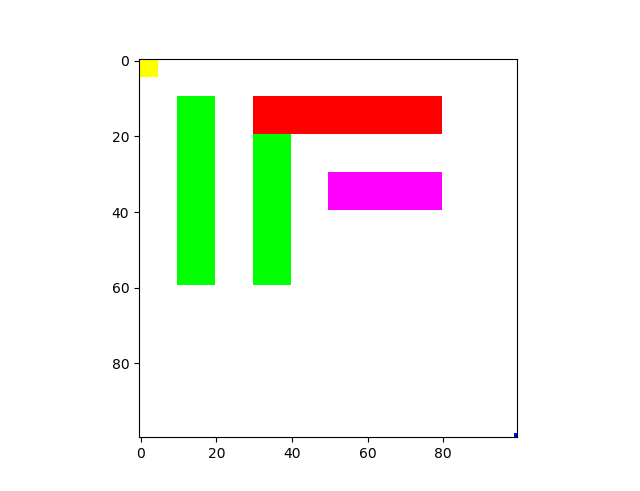
\includegraphics[width=\textwidth]{Figs/env1.png}
        \caption{The robot should pass the green obstacle}
        \label{fig:env1}
    \end{subfigure}%
    \hfill
    \begin{subfigure}[b]{.475\textwidth}
        \centering
        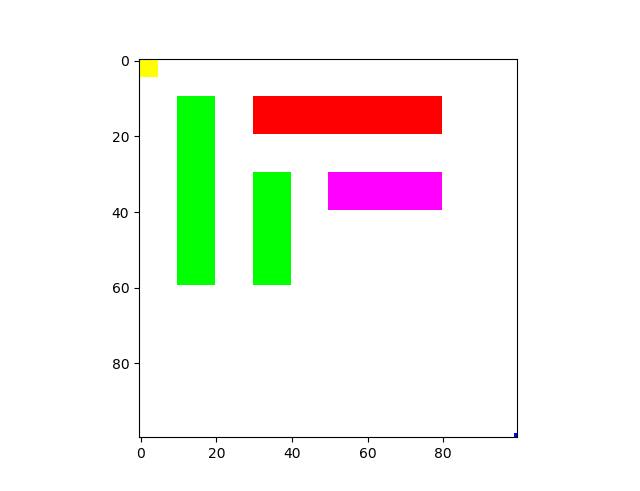
\includegraphics[width=\textwidth]{Figs/env2.png}
        \caption{The robot should avoid the green obstacle}
        \label{fig:env2}
    \end{subfigure}
    \vskip\baselineskip
    \begin{subfigure}[b]{.475\textwidth}
        \centering
        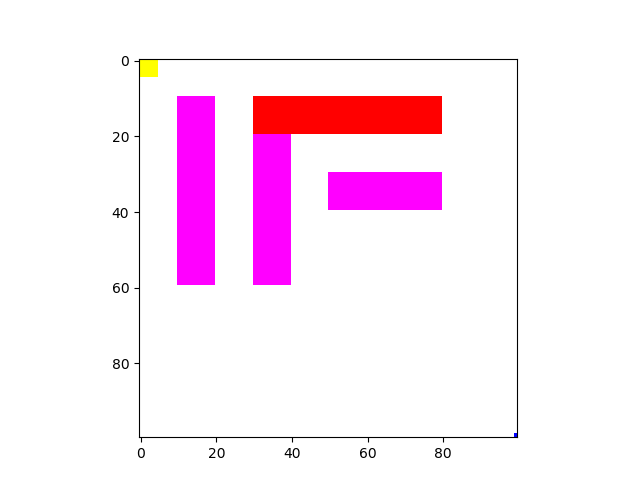
\includegraphics[width=\textwidth]{Figs/env3.png}
        \caption{The robot should choose to detour}
        \label{fig:env3}
    \end{subfigure}%
    \hfill
    \begin{subfigure}[b]{.475\textwidth}
        \centering
        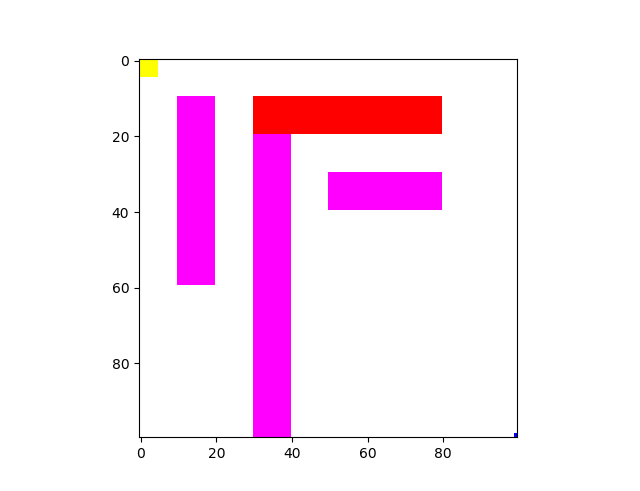
\includegraphics[width=\textwidth]{Figs/env4.png}
        \caption{The robot should pass the purple obstacle}
        \label{fig:env4}
    \end{subfigure}
    \caption{Test environments}
    \label{fig:envs}
\end{figure}

Green color represents obstacles that are easy to pass. 
So the robot should choose to pass the green obstacles if the detour is not too long. (figure \ref{fig:env1} and \ref{fig:env2})

Purple color represents obstacles that are difficult to pass and red color represents obstacles that are impossible to pass.
So the robot should choose to detour around purple obstacles unless the detour is extremely long. (figure \ref{fig:env3} and \ref{fig:env4})
The parameters should be chosen to make the robot make same decisions as indicated in the captions.

\section{Multi-arm robot}
\label{sec:result_project2}


\blankpage
\blankpage

\end{document}